% Options for packages loaded elsewhere
\PassOptionsToPackage{unicode}{hyperref}
\PassOptionsToPackage{hyphens}{url}
%
\documentclass[
]{article}
\usepackage{amsmath,amssymb}
\usepackage{lmodern}
\usepackage{iftex}
\ifPDFTeX
  \usepackage[T1]{fontenc}
  \usepackage[utf8]{inputenc}
  \usepackage{textcomp} % provide euro and other symbols
\else % if luatex or xetex
  \usepackage{unicode-math}
  \defaultfontfeatures{Scale=MatchLowercase}
  \defaultfontfeatures[\rmfamily]{Ligatures=TeX,Scale=1}
\fi
% Use upquote if available, for straight quotes in verbatim environments
\IfFileExists{upquote.sty}{\usepackage{upquote}}{}
\IfFileExists{microtype.sty}{% use microtype if available
  \usepackage[]{microtype}
  \UseMicrotypeSet[protrusion]{basicmath} % disable protrusion for tt fonts
}{}
\makeatletter
\@ifundefined{KOMAClassName}{% if non-KOMA class
  \IfFileExists{parskip.sty}{%
    \usepackage{parskip}
  }{% else
    \setlength{\parindent}{0pt}
    \setlength{\parskip}{6pt plus 2pt minus 1pt}}
}{% if KOMA class
  \KOMAoptions{parskip=half}}
\makeatother
\usepackage{xcolor}
\usepackage[margin=1in]{geometry}
\usepackage{color}
\usepackage{fancyvrb}
\newcommand{\VerbBar}{|}
\newcommand{\VERB}{\Verb[commandchars=\\\{\}]}
\DefineVerbatimEnvironment{Highlighting}{Verbatim}{commandchars=\\\{\}}
% Add ',fontsize=\small' for more characters per line
\usepackage{framed}
\definecolor{shadecolor}{RGB}{248,248,248}
\newenvironment{Shaded}{\begin{snugshade}}{\end{snugshade}}
\newcommand{\AlertTok}[1]{\textcolor[rgb]{0.94,0.16,0.16}{#1}}
\newcommand{\AnnotationTok}[1]{\textcolor[rgb]{0.56,0.35,0.01}{\textbf{\textit{#1}}}}
\newcommand{\AttributeTok}[1]{\textcolor[rgb]{0.77,0.63,0.00}{#1}}
\newcommand{\BaseNTok}[1]{\textcolor[rgb]{0.00,0.00,0.81}{#1}}
\newcommand{\BuiltInTok}[1]{#1}
\newcommand{\CharTok}[1]{\textcolor[rgb]{0.31,0.60,0.02}{#1}}
\newcommand{\CommentTok}[1]{\textcolor[rgb]{0.56,0.35,0.01}{\textit{#1}}}
\newcommand{\CommentVarTok}[1]{\textcolor[rgb]{0.56,0.35,0.01}{\textbf{\textit{#1}}}}
\newcommand{\ConstantTok}[1]{\textcolor[rgb]{0.00,0.00,0.00}{#1}}
\newcommand{\ControlFlowTok}[1]{\textcolor[rgb]{0.13,0.29,0.53}{\textbf{#1}}}
\newcommand{\DataTypeTok}[1]{\textcolor[rgb]{0.13,0.29,0.53}{#1}}
\newcommand{\DecValTok}[1]{\textcolor[rgb]{0.00,0.00,0.81}{#1}}
\newcommand{\DocumentationTok}[1]{\textcolor[rgb]{0.56,0.35,0.01}{\textbf{\textit{#1}}}}
\newcommand{\ErrorTok}[1]{\textcolor[rgb]{0.64,0.00,0.00}{\textbf{#1}}}
\newcommand{\ExtensionTok}[1]{#1}
\newcommand{\FloatTok}[1]{\textcolor[rgb]{0.00,0.00,0.81}{#1}}
\newcommand{\FunctionTok}[1]{\textcolor[rgb]{0.00,0.00,0.00}{#1}}
\newcommand{\ImportTok}[1]{#1}
\newcommand{\InformationTok}[1]{\textcolor[rgb]{0.56,0.35,0.01}{\textbf{\textit{#1}}}}
\newcommand{\KeywordTok}[1]{\textcolor[rgb]{0.13,0.29,0.53}{\textbf{#1}}}
\newcommand{\NormalTok}[1]{#1}
\newcommand{\OperatorTok}[1]{\textcolor[rgb]{0.81,0.36,0.00}{\textbf{#1}}}
\newcommand{\OtherTok}[1]{\textcolor[rgb]{0.56,0.35,0.01}{#1}}
\newcommand{\PreprocessorTok}[1]{\textcolor[rgb]{0.56,0.35,0.01}{\textit{#1}}}
\newcommand{\RegionMarkerTok}[1]{#1}
\newcommand{\SpecialCharTok}[1]{\textcolor[rgb]{0.00,0.00,0.00}{#1}}
\newcommand{\SpecialStringTok}[1]{\textcolor[rgb]{0.31,0.60,0.02}{#1}}
\newcommand{\StringTok}[1]{\textcolor[rgb]{0.31,0.60,0.02}{#1}}
\newcommand{\VariableTok}[1]{\textcolor[rgb]{0.00,0.00,0.00}{#1}}
\newcommand{\VerbatimStringTok}[1]{\textcolor[rgb]{0.31,0.60,0.02}{#1}}
\newcommand{\WarningTok}[1]{\textcolor[rgb]{0.56,0.35,0.01}{\textbf{\textit{#1}}}}
\usepackage{graphicx}
\makeatletter
\def\maxwidth{\ifdim\Gin@nat@width>\linewidth\linewidth\else\Gin@nat@width\fi}
\def\maxheight{\ifdim\Gin@nat@height>\textheight\textheight\else\Gin@nat@height\fi}
\makeatother
% Scale images if necessary, so that they will not overflow the page
% margins by default, and it is still possible to overwrite the defaults
% using explicit options in \includegraphics[width, height, ...]{}
\setkeys{Gin}{width=\maxwidth,height=\maxheight,keepaspectratio}
% Set default figure placement to htbp
\makeatletter
\def\fps@figure{htbp}
\makeatother
\setlength{\emergencystretch}{3em} % prevent overfull lines
\providecommand{\tightlist}{%
  \setlength{\itemsep}{0pt}\setlength{\parskip}{0pt}}
\setcounter{secnumdepth}{-\maxdimen} % remove section numbering
\ifLuaTeX
  \usepackage{selnolig}  % disable illegal ligatures
\fi
\IfFileExists{bookmark.sty}{\usepackage{bookmark}}{\usepackage{hyperref}}
\IfFileExists{xurl.sty}{\usepackage{xurl}}{} % add URL line breaks if available
\urlstyle{same} % disable monospaced font for URLs
\hypersetup{
  pdftitle={homework 3},
  pdfauthor={Yichen Lin},
  hidelinks,
  pdfcreator={LaTeX via pandoc}}

\title{homework 3}
\author{Yichen Lin}
\date{2023-04-04}

\begin{document}
\maketitle

\hypertarget{bike-demand}{%
\subsubsection{1. {[}Bike Demand{]}}\label{bike-demand}}

This problem asks you to visualize a
\href{https://uwmadison.box.com/shared/static/f16jmkkskylfl1hnd5rpslzduja929g2.csv}{dataset}
of hourly bikeshare demand. Provide your code and make sure it is
readable.

\begin{Shaded}
\begin{Highlighting}[]
\NormalTok{bike }\OtherTok{\textless{}{-}} \FunctionTok{read.csv}\NormalTok{(}\StringTok{"https://uwmadison.box.com/shared/static/f16jmkkskylfl1hnd5rpslzduja929g2.csv"}\NormalTok{)}
\FunctionTok{head}\NormalTok{(bike)}
\end{Highlighting}
\end{Shaded}

\begin{verbatim}
##       dteday season yr mnth hr holiday weekday temp  hum windspeed count
## 1 2011-01-01      1  0    1  0       0       6 0.24 0.81    0.0000    16
## 2 2011-01-01      1  0    1  1       0       6 0.22 0.80    0.0000    40
## 3 2011-01-01      1  0    1  2       0       6 0.22 0.80    0.0000    32
## 4 2011-01-01      1  0    1  3       0       6 0.24 0.75    0.0000    13
## 5 2011-01-01      1  0    1  4       0       6 0.24 0.75    0.0000     1
## 6 2011-01-01      1  0    1  5       0       6 0.24 0.75    0.0896     1
\end{verbatim}

\begin{enumerate}
\def\labelenumi{\alph{enumi}.}
\tightlist
\item
  Make a line plot of bike demand (\texttt{count}) by hour, faceted out
  across the 7 days of the week (\texttt{weekday}).
\end{enumerate}

\begin{Shaded}
\begin{Highlighting}[]
\NormalTok{line\_plot }\OtherTok{\textless{}{-}}  \FunctionTok{ggplot}\NormalTok{(bike) }\SpecialCharTok{+}
  \FunctionTok{geom\_line}\NormalTok{(}\FunctionTok{aes}\NormalTok{(}\AttributeTok{x =}\NormalTok{ hr, }\AttributeTok{y =}\NormalTok{ count, }\AttributeTok{group =}\NormalTok{ dteday)) }\SpecialCharTok{+}
  \FunctionTok{facet\_wrap}\NormalTok{(}\SpecialCharTok{\textasciitilde{}}\NormalTok{ weekday)}

\NormalTok{line\_plot}
\end{Highlighting}
\end{Shaded}

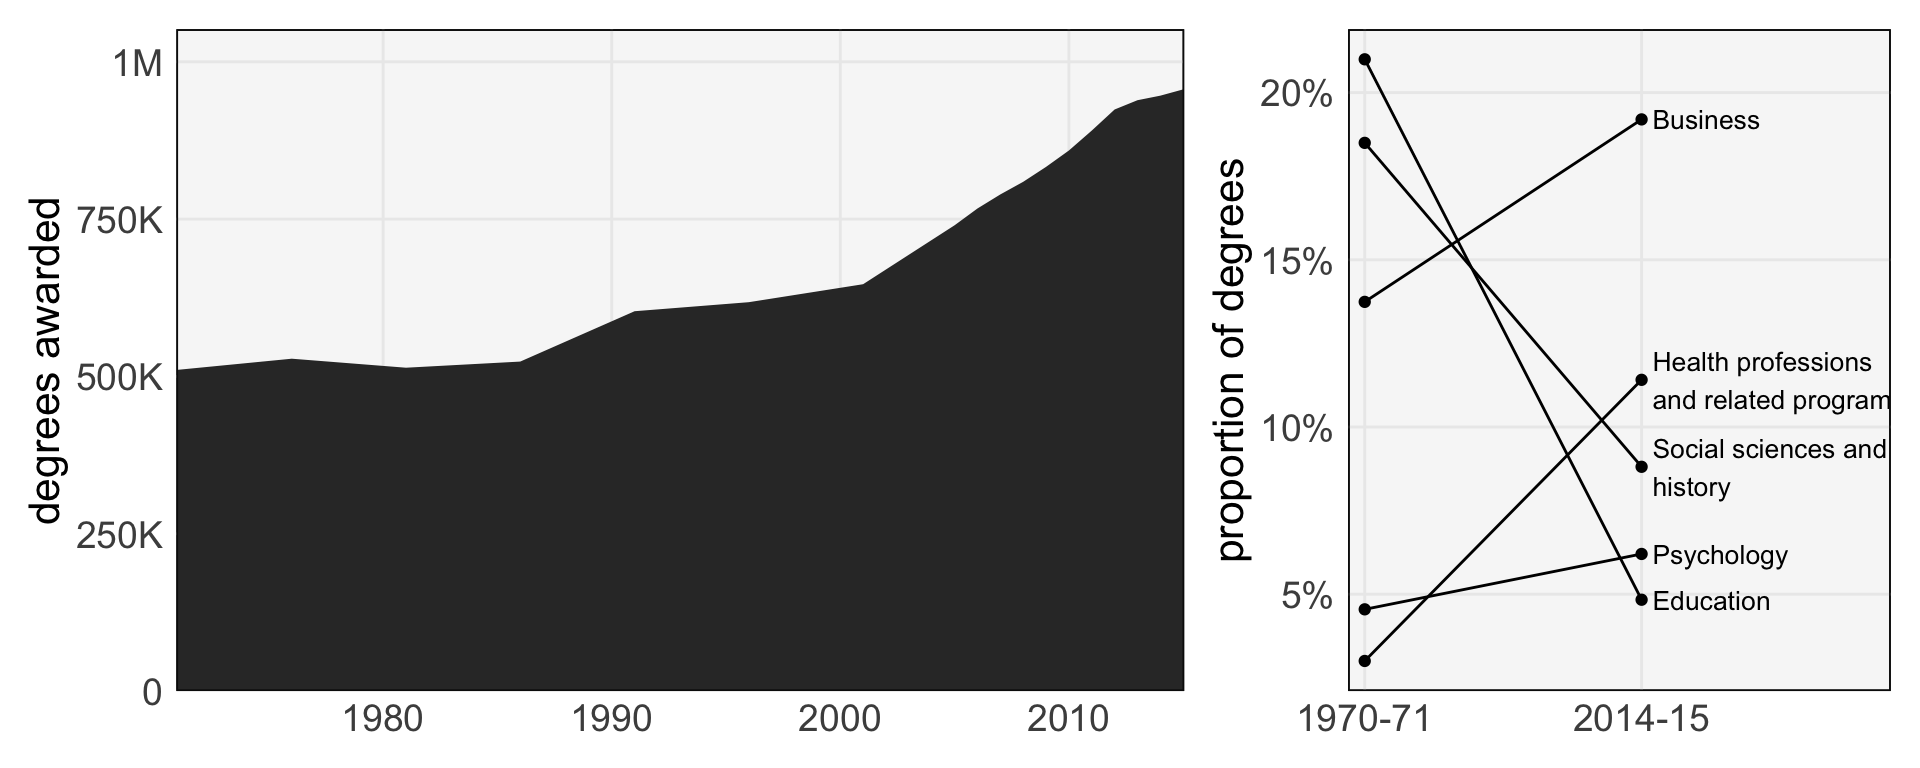
\includegraphics{hw3_files/figure-latex/unnamed-chunk-2-1.pdf}

\begin{enumerate}
\def\labelenumi{\alph{enumi}.}
\setcounter{enumi}{1}
\tightlist
\item
  Create a new summary data.frame giving the 25 and 75 percent quantiles
  of demand (\texttt{count}) for each hour (\texttt{hr}) by day of the
  week (\texttt{weekday}) combination, separately within each year
  (\texttt{yr}) that the data was collected.
\end{enumerate}

\begin{Shaded}
\begin{Highlighting}[]
\NormalTok{new\_summary }\OtherTok{\textless{}{-}}\NormalTok{ bike }\SpecialCharTok{\%\textgreater{}\%}
  \FunctionTok{group\_by}\NormalTok{(yr,weekday,hr) }\SpecialCharTok{\%\textgreater{}\%}
  \FunctionTok{summarise}\NormalTok{(}\AttributeTok{q25 =} \FunctionTok{quantile}\NormalTok{(count,}\FloatTok{0.25}\NormalTok{,}\AttributeTok{na.rm =} \ConstantTok{TRUE}\NormalTok{),}
            \AttributeTok{q75 =} \FunctionTok{quantile}\NormalTok{(count,}\FloatTok{0.75}\NormalTok{,}\AttributeTok{na.rm =} \ConstantTok{TRUE}\NormalTok{))}

\NormalTok{new\_summary}
\end{Highlighting}
\end{Shaded}

\begin{verbatim}
## # A tibble: 336 x 5
## # Groups:   yr, weekday [14]
##       yr weekday    hr   q25   q75
##    <int>   <int> <int> <dbl> <dbl>
##  1     0       0     0  39   108. 
##  2     0       0     1  33.5  79  
##  3     0       0     2  29    65.8
##  4     0       0     3  13.5  35  
##  5     0       0     4   3    11  
##  6     0       0     5   4     9  
##  7     0       0     6   3    16.8
##  8     0       0     7  10    37.2
##  9     0       0     8  33.5  92  
## 10     0       0     9  58   172. 
## # i 326 more rows
\end{verbatim}

\begin{enumerate}
\def\labelenumi{\alph{enumi}.}
\setcounter{enumi}{2}
\tightlist
\item
  Using a ribbon plot, overlay the quantities from (b) onto your plot
  from part (a). Use color to distinguish between the ribbons for the
  first and second year that the data were collected.
\end{enumerate}

\begin{Shaded}
\begin{Highlighting}[]
\NormalTok{line\_plot }\SpecialCharTok{+}
  \FunctionTok{geom\_ribbon}\NormalTok{(}\AttributeTok{data =}\NormalTok{ new\_summary, }
              \FunctionTok{aes}\NormalTok{(}\AttributeTok{x =}\NormalTok{ hr, }\AttributeTok{ymin =}\NormalTok{ q25, }\AttributeTok{ymax =}\NormalTok{ q75, }\AttributeTok{fill =} \FunctionTok{as.factor}\NormalTok{(yr))) }\SpecialCharTok{+}
  \FunctionTok{scale\_fill\_manual}\NormalTok{(}\AttributeTok{values =} \FunctionTok{c}\NormalTok{(}\StringTok{"red"}\NormalTok{, }\StringTok{"blue"}\NormalTok{))}
\end{Highlighting}
\end{Shaded}

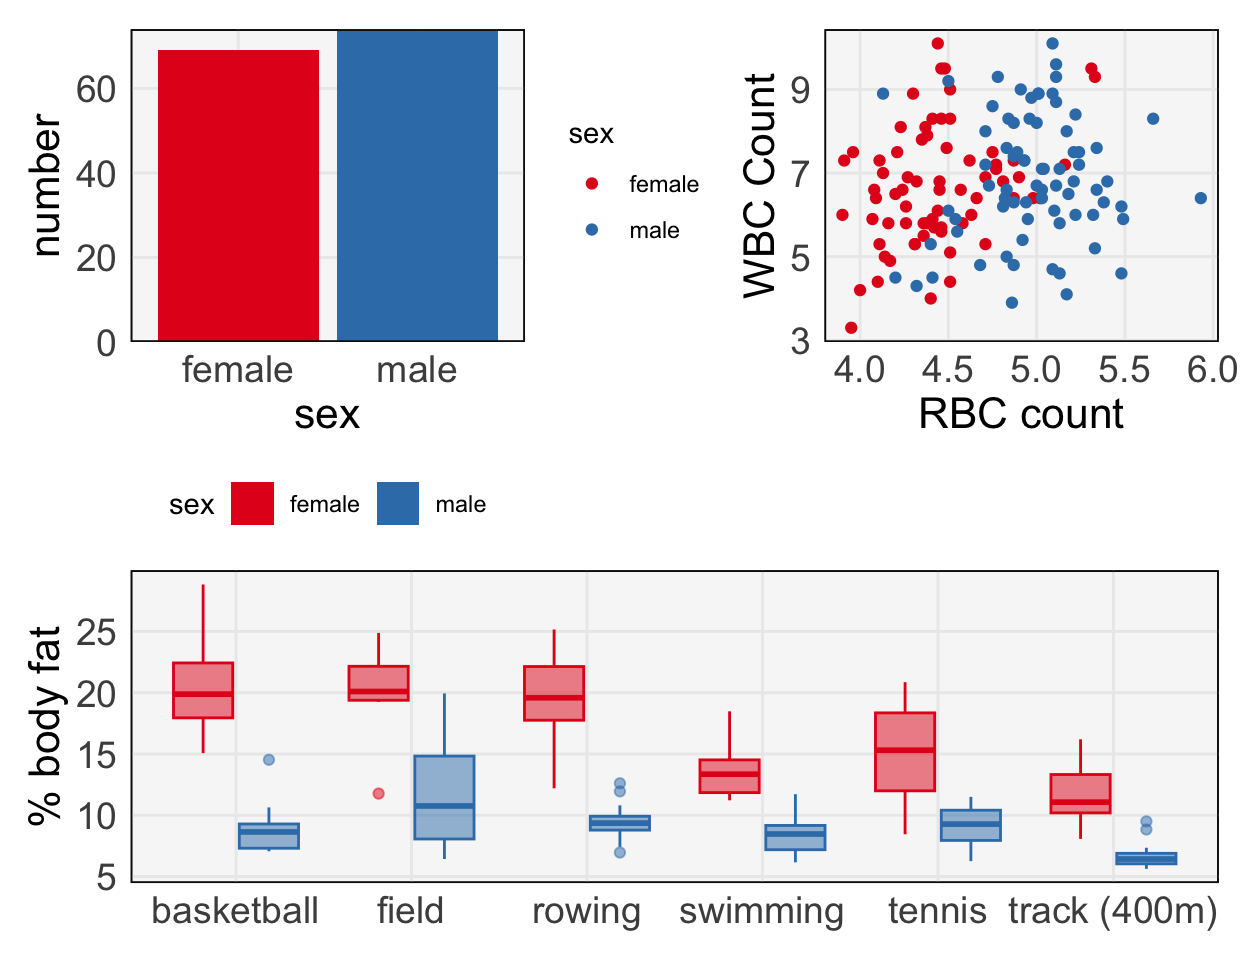
\includegraphics{hw3_files/figure-latex/unnamed-chunk-4-1.pdf}

\begin{enumerate}
\def\labelenumi{\alph{enumi}.}
\setcounter{enumi}{3}
\tightlist
\item
  Provide a brief description of some takeaways from the final
  visualization.
\end{enumerate}

For weekdays, there are two strong cyclics at about 7:30 a.m and 17:30
p.m., which corresponds to people's work hours. During weekend, usage
dema nd gradually increases in the morning, reaches its peak at noon,
and then gradually decreases.

\hypertarget{calfresh-enrollment-i}{%
\subsubsection{2. {[}CalFresh Enrollment
I{]}}\label{calfresh-enrollment-i}}

In this problem, we will investigate spatial and temporal aspects of
enrollment in CalFresh, a nutritional assistance program in California.

\begin{enumerate}
\def\labelenumi{\alph{enumi}.}
\tightlist
\item
  The code below reads in the CalFresh data. We've filtered out February
  2019, since benefits were distributed differently in this month,
  leading to outliers for most counties. Extract features of the
  \texttt{calfresh} time series using the \texttt{features} function in
  the feasts library.
\end{enumerate}

\begin{Shaded}
\begin{Highlighting}[]
\FunctionTok{library}\NormalTok{(tsibble)}
\NormalTok{calfresh }\OtherTok{\textless{}{-}} \FunctionTok{read.csv}\NormalTok{(}\StringTok{"https://uwmadison.box.com/shared/static/rduej9hsc4w3mdethxnx9ccv752f22yr.csv"}\NormalTok{) }\SpecialCharTok{\%\textgreater{}\%}
  \FunctionTok{filter}\NormalTok{(date }\SpecialCharTok{!=} \StringTok{"2019 Feb"}\NormalTok{) }\SpecialCharTok{\%\textgreater{}\%}
  \FunctionTok{mutate}\NormalTok{(}\AttributeTok{date =} \FunctionTok{yearmonth}\NormalTok{(date)) }\SpecialCharTok{\%\textgreater{}\%}
  \FunctionTok{as\_tsibble}\NormalTok{(}\AttributeTok{key =}\NormalTok{ county, }\AttributeTok{index =}\NormalTok{ date)}

\NormalTok{calfresh }
\end{Highlighting}
\end{Shaded}

\begin{verbatim}
## # A tsibble: 4,872 x 5 [1M]
## # Key:       county [58]
##    county      date medi_cal unemployment calfresh
##    <chr>      <mth> <chr>           <dbl>    <int>
##  1 Alameda 2014 Jan 340 549           6.5    64394
##  2 Alameda 2014 Feb 349 927           6.4    63674
##  3 Alameda 2014 Mar 365 622           6.4    64297
##  4 Alameda 2014 Apr 373 571           5.5    64208
##  5 Alameda 2014 May 378 218           5.6    64582
##  6 Alameda 2014 Jun 381 831           5.9    64635
##  7 Alameda 2014 Jul 385 839           6.3    64020
##  8 Alameda 2014 Aug 389 814           6.1    63835
##  9 Alameda 2014 Sep 393 082           5.5    63346
## 10 Alameda 2014 Oct 396 515           5.4    63146
## # i 4,862 more rows
\end{verbatim}

\begin{Shaded}
\begin{Highlighting}[]
\NormalTok{calf }\OtherTok{\textless{}{-}}\NormalTok{ calfresh }\SpecialCharTok{\%\textgreater{}\%}
  \FunctionTok{features}\NormalTok{(calfresh, }\AttributeTok{features =} \FunctionTok{feature\_set}\NormalTok{(}\AttributeTok{tag =} \StringTok{"trend"}\NormalTok{),}\AttributeTok{na.rm =} \ConstantTok{TRUE}\NormalTok{) }\SpecialCharTok{\%\textgreater{}\%}
  \FunctionTok{left\_join}\NormalTok{(calfresh,}\AttributeTok{by =} \StringTok{"county"}\NormalTok{)}

\NormalTok{calf}
\end{Highlighting}
\end{Shaded}

\begin{verbatim}
## # A tibble: 4,872 x 14
##    county  trend_strength seasonal_strength_year seasonal_peak_year
##    <chr>            <dbl>                  <dbl>              <dbl>
##  1 Alameda          0.929                  0.321                  5
##  2 Alameda          0.929                  0.321                  5
##  3 Alameda          0.929                  0.321                  5
##  4 Alameda          0.929                  0.321                  5
##  5 Alameda          0.929                  0.321                  5
##  6 Alameda          0.929                  0.321                  5
##  7 Alameda          0.929                  0.321                  5
##  8 Alameda          0.929                  0.321                  5
##  9 Alameda          0.929                  0.321                  5
## 10 Alameda          0.929                  0.321                  5
## # i 4,862 more rows
## # i 10 more variables: seasonal_trough_year <dbl>, spikiness <dbl>,
## #   linearity <dbl>, curvature <dbl>, stl_e_acf1 <dbl>, stl_e_acf10 <dbl>,
## #   date <mth>, medi_cal <chr>, unemployment <dbl>, calfresh <int>
\end{verbatim}

\begin{enumerate}
\def\labelenumi{\alph{enumi}.}
\setcounter{enumi}{1}
\tightlist
\item
  Visualize CalFresh enrollment over time for the counties with the
  highest and lowest \texttt{seasonal\_strength\_year}.
\end{enumerate}

\begin{Shaded}
\begin{Highlighting}[]
\NormalTok{calf }\SpecialCharTok{\%\textgreater{}\%}
  \FunctionTok{group\_by}\NormalTok{(county) }\SpecialCharTok{\%\textgreater{}\%}
  \FunctionTok{filter}\NormalTok{(seasonal\_strength\_year }\SpecialCharTok{==} \FunctionTok{max}\NormalTok{(seasonal\_strength\_year)) }\SpecialCharTok{\%\textgreater{}\%}
  \FunctionTok{pull}\NormalTok{(county) }\OtherTok{{-}\textgreater{}}\NormalTok{ highest\_county}

\NormalTok{calf }\SpecialCharTok{\%\textgreater{}\%}
  \FunctionTok{group\_by}\NormalTok{(county) }\SpecialCharTok{\%\textgreater{}\%}
  \FunctionTok{filter}\NormalTok{(seasonal\_strength\_year }\SpecialCharTok{==} \FunctionTok{min}\NormalTok{(seasonal\_strength\_year)) }\SpecialCharTok{\%\textgreater{}\%}
  \FunctionTok{pull}\NormalTok{(county) }\OtherTok{{-}\textgreater{}}\NormalTok{ lowest\_county}

\NormalTok{Calfresh\_enrollment }\OtherTok{\textless{}{-}}\NormalTok{ calf }\SpecialCharTok{\%\textgreater{}\%}
  \FunctionTok{filter}\NormalTok{(county }\SpecialCharTok{\%in\%} \FunctionTok{c}\NormalTok{(highest\_county,lowest\_county)) }\SpecialCharTok{\%\textgreater{}\%}
  \FunctionTok{ggplot}\NormalTok{(}\FunctionTok{aes}\NormalTok{(}\AttributeTok{x =}\NormalTok{ date, }\AttributeTok{y =}\NormalTok{ calfresh, }\AttributeTok{col =}\NormalTok{ county)) }\SpecialCharTok{+}
  \FunctionTok{geom\_line}\NormalTok{() }\SpecialCharTok{+}
  \FunctionTok{labs}\NormalTok{(}\AttributeTok{x =} \StringTok{"time"}\NormalTok{, }\AttributeTok{y =} \StringTok{"calfresh enrollment"}\NormalTok{,}
       \AttributeTok{title =} \StringTok{"calfresh enrollment over time for the counties with the highest and}
\StringTok{    lowest \textasciigrave{}seasonal\_strength\_year\textasciigrave{}"}\NormalTok{)}

\NormalTok{Calfresh\_enrollment}
\end{Highlighting}
\end{Shaded}

\begin{verbatim}
## Warning: Removed 58 rows containing missing values (`geom_line()`).
\end{verbatim}

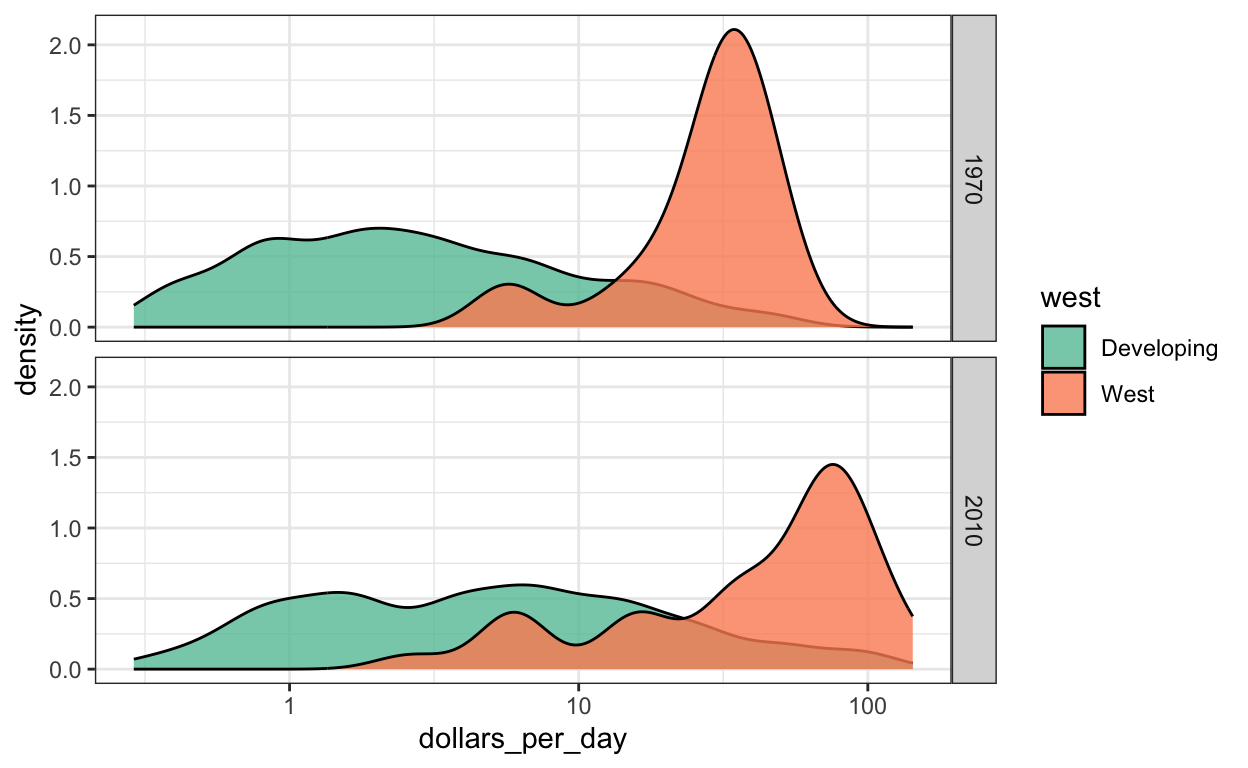
\includegraphics{hw3_files/figure-latex/unnamed-chunk-7-1.pdf}

\begin{enumerate}
\def\labelenumi{\alph{enumi}.}
\setcounter{enumi}{2}
\tightlist
\item
  The code below reads in a vector dataset demarcating the county
  boundaries in California. Join in the features dataset from (a) with
  this these vector data. Use this to produce a map with each county
  shaded in by its \texttt{seasonal\_strength\_year}.
\end{enumerate}

\begin{Shaded}
\begin{Highlighting}[]
\FunctionTok{library}\NormalTok{(sf)}
\NormalTok{counties }\OtherTok{\textless{}{-}} \FunctionTok{read\_sf}\NormalTok{(}\StringTok{"https://uwmadison.box.com/shared/static/gropucqxgqm82yhq13do1ws9k16dnxq7.geojson"}\NormalTok{)}
\NormalTok{joint\_calf }\OtherTok{\textless{}{-}} \FunctionTok{left\_join}\NormalTok{(counties,calf,}\AttributeTok{by =} \StringTok{"county"}\NormalTok{)}
\NormalTok{joint\_calf}
\end{Highlighting}
\end{Shaded}

\begin{verbatim}
## Simple feature collection with 4872 features and 14 fields
## Geometry type: MULTIPOLYGON
## Dimension:     XY
## Bounding box:  xmin: -124.4087 ymin: 32.53429 xmax: -114.1312 ymax: 42.00952
## Geodetic CRS:  WGS 84
## # A tibble: 4,872 x 15
##    county                         geometry trend_strength seasonal_strength_year
##    <chr>                <MULTIPOLYGON [°]>          <dbl>                  <dbl>
##  1 Alameda (((-122.3129 37.89733, -122.28~          0.929                  0.321
##  2 Alameda (((-122.3129 37.89733, -122.28~          0.929                  0.321
##  3 Alameda (((-122.3129 37.89733, -122.28~          0.929                  0.321
##  4 Alameda (((-122.3129 37.89733, -122.28~          0.929                  0.321
##  5 Alameda (((-122.3129 37.89733, -122.28~          0.929                  0.321
##  6 Alameda (((-122.3129 37.89733, -122.28~          0.929                  0.321
##  7 Alameda (((-122.3129 37.89733, -122.28~          0.929                  0.321
##  8 Alameda (((-122.3129 37.89733, -122.28~          0.929                  0.321
##  9 Alameda (((-122.3129 37.89733, -122.28~          0.929                  0.321
## 10 Alameda (((-122.3129 37.89733, -122.28~          0.929                  0.321
## # i 4,862 more rows
## # i 11 more variables: seasonal_peak_year <dbl>, seasonal_trough_year <dbl>,
## #   spikiness <dbl>, linearity <dbl>, curvature <dbl>, stl_e_acf1 <dbl>,
## #   stl_e_acf10 <dbl>, date <mth>, medi_cal <chr>, unemployment <dbl>,
## #   calfresh <int>
\end{verbatim}

\begin{Shaded}
\begin{Highlighting}[]
\FunctionTok{ggplot}\NormalTok{(joint\_calf) }\SpecialCharTok{+}
  \FunctionTok{geom\_sf}\NormalTok{(}\FunctionTok{aes}\NormalTok{(}\AttributeTok{fill =}\NormalTok{ seasonal\_strength\_year,}\AttributeTok{geometry =}\NormalTok{ geometry),}
          \AttributeTok{col =} \StringTok{"black"}\NormalTok{, }\AttributeTok{lwd =} \FloatTok{0.2}\NormalTok{, }\AttributeTok{lty =} \DecValTok{2}\NormalTok{) }\SpecialCharTok{+}
  \FunctionTok{scale\_fill\_gradient}\NormalTok{(}\AttributeTok{low =} \StringTok{"white"}\NormalTok{,}\AttributeTok{high =} \StringTok{"steelblue"}\NormalTok{) }\SpecialCharTok{+}
  \FunctionTok{labs}\NormalTok{(}\AttributeTok{title =} \StringTok{"Seasonal strength year"}\NormalTok{)}
\end{Highlighting}
\end{Shaded}

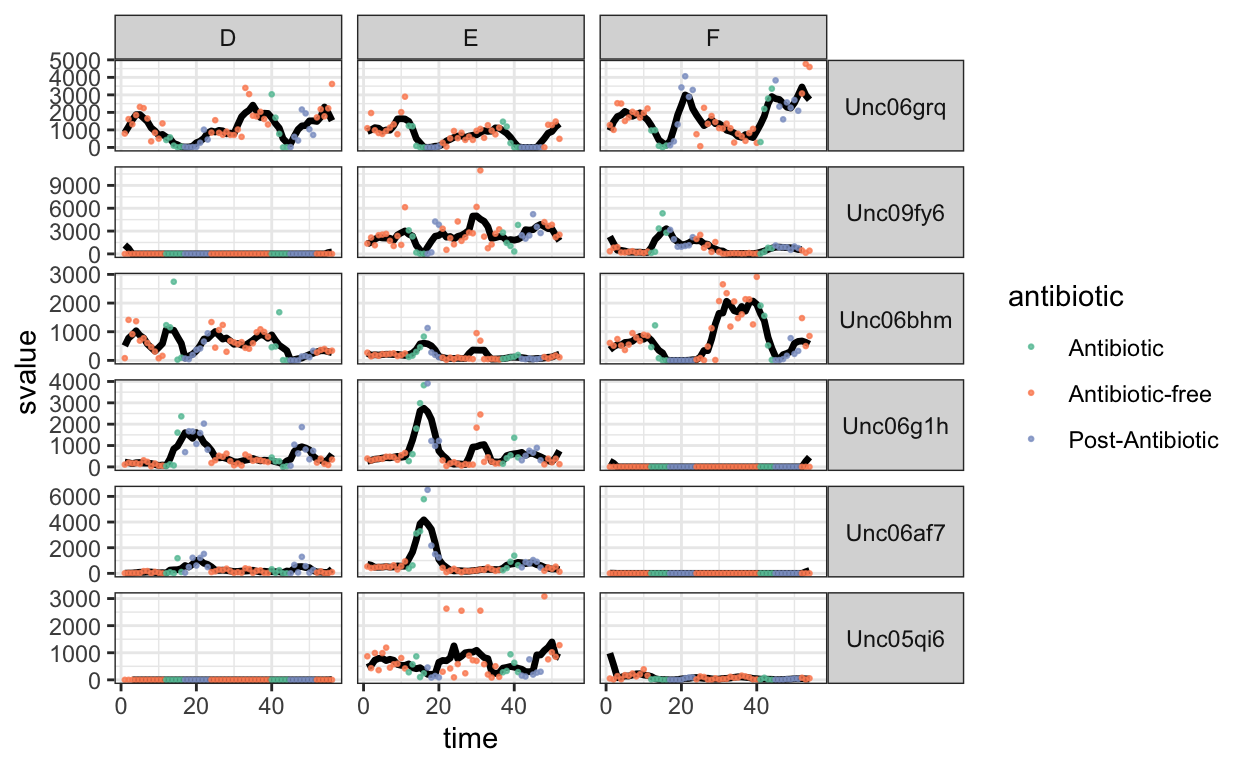
\includegraphics{hw3_files/figure-latex/unnamed-chunk-9-1.pdf}

\begin{verbatim}
d. Propose, but do not implement, a visualization of this dataset that makes use
of dynamic queries. What questions would the visualization answer? What would be
the structure of interaction, and how would the display update when the user
provides a cue?

As a spatial and temporal data set, visualization of it can answer question like 
the background of certain county, how the enrollment of this program change over 
time in certain county. The users can choose those county that they want to explore 
on the map, and a line plot and a table will show information of chosen county.
\end{verbatim}

\hypertarget{political-book-recommendations}{%
\subsubsection{3. {[}Political Book
Recommendations{]}}\label{political-book-recommendations}}

In this problem, we'll study a network dataset of Amazon bestselling US
Politics books. Books are linked by an edge if they appeared together in
the recommendations (``customers who bought this book also bought these
other books'').

\begin{enumerate}
\def\labelenumi{\alph{enumi}.}
\tightlist
\item
  The code below reads in the edges and nodes associated with the
  network. The edges dataset only contains IDs of co-recommended books,
  while the nodes data includes attributes associated with each book.
  Build a \texttt{tbl\_graph} object to store the graph.
\end{enumerate}

\begin{Shaded}
\begin{Highlighting}[]
\NormalTok{edges }\OtherTok{\textless{}{-}} \FunctionTok{read\_csv}\NormalTok{(}\StringTok{"https://raw.githubusercontent.com/krisrs1128/stat679\_code/main/activities/week10/political{-}books{-}edges.csv"}\NormalTok{, }\AttributeTok{col\_types =} \StringTok{"cci"}\NormalTok{)}
\NormalTok{nodes }\OtherTok{\textless{}{-}} \FunctionTok{read\_csv}\NormalTok{(}\StringTok{"https://raw.githubusercontent.com/krisrs1128/stat679\_code/main/activities/week10/political{-}books{-}nodes.csv"}\NormalTok{, }\AttributeTok{col\_types =} \StringTok{"ccc"}\NormalTok{)}
\end{Highlighting}
\end{Shaded}

\begin{Shaded}
\begin{Highlighting}[]
\NormalTok{graph }\OtherTok{\textless{}{-}} \FunctionTok{tbl\_graph}\NormalTok{(nodes, edges, }\AttributeTok{directed =} \ConstantTok{FALSE}\NormalTok{)}
\NormalTok{graph}
\end{Highlighting}
\end{Shaded}

\begin{verbatim}
## # A tbl_graph: 105 nodes and 441 edges
## #
## # An undirected simple graph with 1 component
## #
## # A tibble: 105 x 3
##   id    label                      political_ideology
##   <chr> <chr>                      <chr>             
## 1 0     1000 Years for Revenge     neutral           
## 2 1     Bush vs. the Beltway       conservative      
## 3 2     Charlie Wilson's War       conservative      
## 4 3     Losing Bin Laden           conservative      
## 5 4     Sleeping With the Devil    neutral           
## 6 5     The Man Who Warned America conservative      
## # i 99 more rows
## #
## # A tibble: 441 x 3
##    from    to weight
##   <int> <int>  <int>
## 1     1     2      1
## 2     1     3      1
## 3     1     4      1
## # i 438 more rows
\end{verbatim}

\begin{enumerate}
\def\labelenumi{\alph{enumi}.}
\setcounter{enumi}{1}
\tightlist
\item
  Use the result from part (a) to visualize the network as a node-link
  diagram. Include the book's title in the node label, and shade in the
  node according to political ideology.
\end{enumerate}

\begin{Shaded}
\begin{Highlighting}[]
\NormalTok{nodes}
\end{Highlighting}
\end{Shaded}

\begin{verbatim}
## # A tibble: 105 x 3
##    id    label                      political_ideology
##    <chr> <chr>                      <chr>             
##  1 0     1000 Years for Revenge     neutral           
##  2 1     Bush vs. the Beltway       conservative      
##  3 2     Charlie Wilson's War       conservative      
##  4 3     Losing Bin Laden           conservative      
##  5 4     Sleeping With the Devil    neutral           
##  6 5     The Man Who Warned America conservative      
##  7 6     Why America Slept          neutral           
##  8 7     Ghost Wars                 neutral           
##  9 8     A National Party No More   conservative      
## 10 9     Bush Country               conservative      
## # i 95 more rows
\end{verbatim}

\begin{Shaded}
\begin{Highlighting}[]
\CommentTok{\# ggraph(graph,layout = "kk") +}
\CommentTok{\#   geom\_edge\_link() +}
\CommentTok{\#   geom\_node\_label(aes(label = nodes$label),repel = TRUE) +}
\CommentTok{\#   geom\_node\_point(aes(color = political\_ideology))}
\end{Highlighting}
\end{Shaded}

Due to the limitation of figure size, the screenshot of the figure is as
follows: 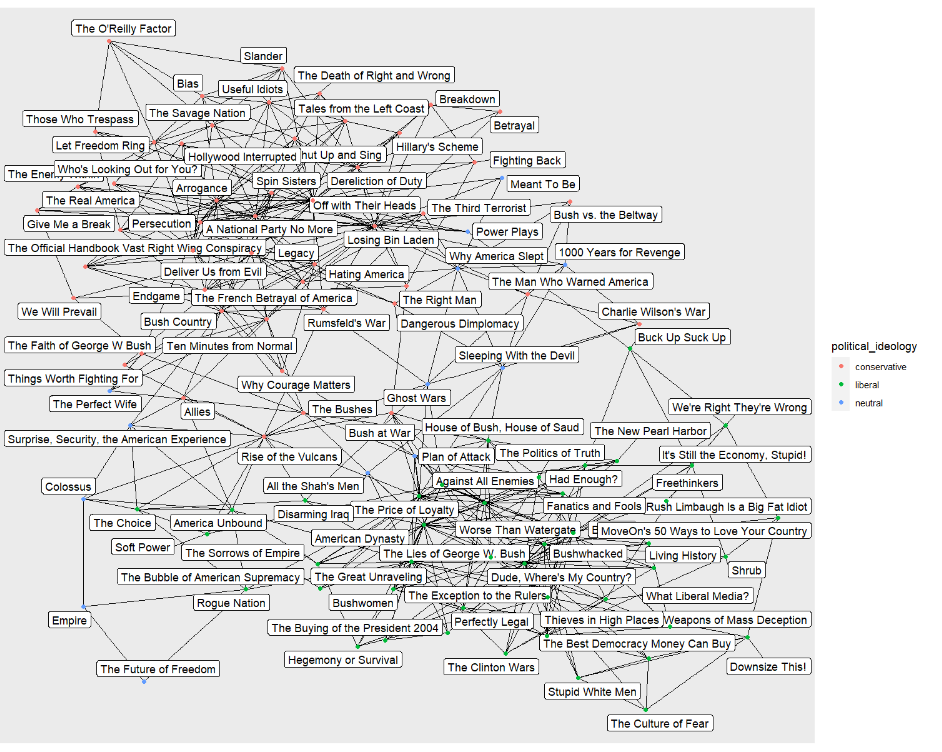
\includegraphics{graph.png}

\begin{enumerate}
\def\labelenumi{\alph{enumi}.}
\setcounter{enumi}{2}
\tightlist
\item
  Create the analogous adjacency matrix visualization. Provide examples
  of visual queries that are easy to answer using one encoding but not
  the other (i.e., what is easy to see in the node-link view vs.~what is
  easy to see in the adjacency matrix).
\end{enumerate}

The visualization is as follows. One example query is that whether it is
an inner group or structure within each political ideology. From the
output below, there are two or three groups within ``conservative''
books. And for ``liberal'' books, there is one big group. Another
interesting finding is that from the visualization of the adjacency
matrix, books labeled with ``neutral'' are less likely to connected with
each other.

\begin{Shaded}
\begin{Highlighting}[]
\FunctionTok{ggraph}\NormalTok{(graph, }\StringTok{"matrix"}\NormalTok{) }\SpecialCharTok{+}
  \FunctionTok{geom\_node\_point}\NormalTok{(}\FunctionTok{aes}\NormalTok{(}\AttributeTok{col =}\NormalTok{ political\_ideology), }\AttributeTok{x =} \SpecialCharTok{{-}}\DecValTok{1}\NormalTok{) }\SpecialCharTok{+}
  \FunctionTok{geom\_node\_point}\NormalTok{(}\FunctionTok{aes}\NormalTok{(}\AttributeTok{col =}\NormalTok{ political\_ideology), }\AttributeTok{y =} \DecValTok{1}\NormalTok{) }\SpecialCharTok{+}
  \FunctionTok{geom\_edge\_tile}\NormalTok{(}\AttributeTok{mirror =} \ConstantTok{TRUE}\NormalTok{) }\SpecialCharTok{+}
  \FunctionTok{scale\_y\_reverse}\NormalTok{() }\SpecialCharTok{+}
  \FunctionTok{scale\_color\_brewer}\NormalTok{(}\AttributeTok{palette =} \StringTok{"Set1"}\NormalTok{) }\SpecialCharTok{+}
  \FunctionTok{labs}\NormalTok{(}\AttributeTok{title =} \StringTok{"Amazon bestselling US Politics books"}\NormalTok{)}
\end{Highlighting}
\end{Shaded}

\begin{verbatim}
## Warning: Using the `size` aesthetic in this geom was deprecated in ggplot2 3.4.0.
## i Please use `linewidth` in the `default_aes` field and elsewhere instead.
## This warning is displayed once every 8 hours.
## Call `lifecycle::last_lifecycle_warnings()` to see where this warning was
## generated.
\end{verbatim}

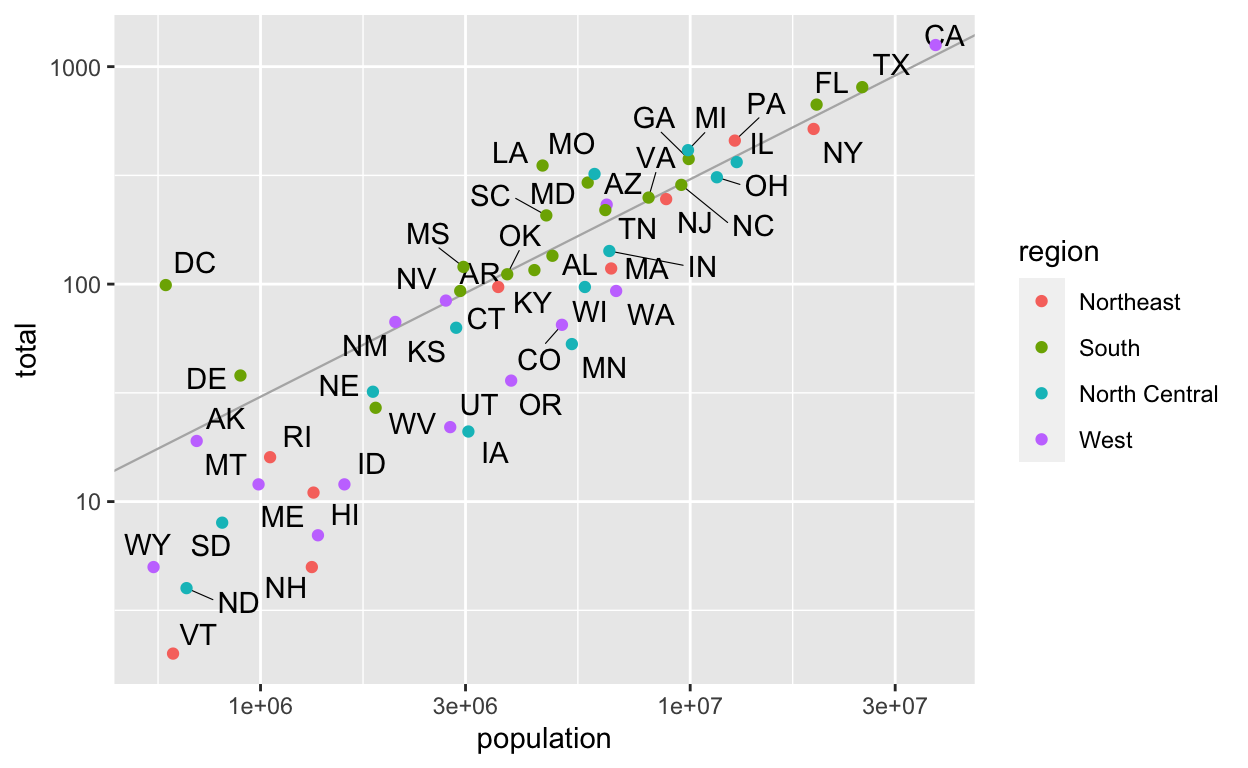
\includegraphics{hw3_files/figure-latex/unnamed-chunk-14-1.pdf}

\begin{Shaded}
\begin{Highlighting}[]
  \FunctionTok{coord\_fixed}\NormalTok{()}
\end{Highlighting}
\end{Shaded}

\begin{verbatim}
## <ggproto object: Class CoordFixed, CoordCartesian, Coord, gg>
##     aspect: function
##     backtransform_range: function
##     clip: on
##     default: FALSE
##     distance: function
##     expand: TRUE
##     is_free: function
##     is_linear: function
##     labels: function
##     limits: list
##     modify_scales: function
##     range: function
##     ratio: 1
##     render_axis_h: function
##     render_axis_v: function
##     render_bg: function
##     render_fg: function
##     setup_data: function
##     setup_layout: function
##     setup_panel_guides: function
##     setup_panel_params: function
##     setup_params: function
##     train_panel_guides: function
##     transform: function
##     super:  <ggproto object: Class CoordFixed, CoordCartesian, Coord, gg>
\end{verbatim}

\hypertarget{nyc-rentals}{%
\subsubsection{4. {[}NYC Rentals{]}}\label{nyc-rentals}}

In this problem, we'll create a visualization to dynamically query a
\href{https://uwmadison.box.com/shared/static/zi72ugnpku714rbqo2og9tv2yib5xped.csv}{dataset}
of Airbnb rentals in Manhattan in 2019. The steps below guide you
through the process of building this visualization.

\begin{enumerate}
\def\labelenumi{\alph{enumi}.}
\tightlist
\item
  Make a scatterplot of locations (Longitude vs.~Latitude) for all the
  rentals, colored in by \texttt{room\_type}.
\end{enumerate}

\begin{Shaded}
\begin{Highlighting}[]
\NormalTok{NYCrentals }\OtherTok{\textless{}{-}} \FunctionTok{read.csv}\NormalTok{(}\StringTok{"https://uwmadison.box.com/shared/static/zi72ugnpku714rbqo2og9tv2yib5xped.csv"}\NormalTok{)}
\FunctionTok{head}\NormalTok{(NYCrentals)}
\end{Highlighting}
\end{Shaded}

\begin{verbatim}
##         id                                               name   host_id
## 1  2619549                Charming, Modern 2BR | Central Park  13347167
## 2 34291583           Sonder | 116 John | Relaxed Studio + Gym 219517861
## 3 16427854       Trendy 1 bedroom apartment in cool LES hood.  83185960
## 4 23901975 BrightClean Studio near Grand Central (MurrayHill)  43275413
## 5 10132356            Giant Loft with a Huge Deck and Kitchen  21247379
## 6  3613839                  Cozy  and sunny room in Manhattan  17450462
##        host_name neighbourhood_group      neighbourhood latitude longitude
## 1 AFI Apartments           Manhattan    Upper East Side 40.77265 -73.95740
## 2   Sonder (NYC)           Manhattan Financial District 40.70838 -74.00694
## 3        Dr. Amy           Manhattan    Lower East Side 40.71510 -73.98661
## 4         Ashumi           Manhattan            Midtown 40.74640 -73.97987
## 5           Paul           Manhattan             Harlem 40.80926 -73.95455
## 6         Esther           Manhattan             Harlem 40.82544 -73.94020
##         room_type price minimum_nights number_of_reviews last_review
## 1 Entire home/apt   140             30                 1  2018-09-30
## 2 Entire home/apt   100             29                 0        <NA>
## 3 Entire home/apt   180              3                49  2019-05-28
## 4 Entire home/apt   180              2                18  2019-06-02
## 5 Entire home/apt   150              3                25  2019-06-14
## 6    Private room    60              7                45  2019-06-09
##   reviews_per_month calculated_host_listings_count availability_365 log_price
## 1              0.11                             29              329  4.941642
## 2                NA                            327              351  4.605170
## 3              1.58                              1                1  5.192957
## 4              1.22                              1                4  5.192957
## 5              1.20                              1               22  5.010635
## 6              0.92                              1              290  4.094345
\end{verbatim}

\begin{Shaded}
\begin{Highlighting}[]
\FunctionTok{ggplot}\NormalTok{(NYCrentals) }\SpecialCharTok{+}
  \FunctionTok{geom\_point}\NormalTok{(}\FunctionTok{aes}\NormalTok{(}\AttributeTok{x =}\NormalTok{ longitude, }\AttributeTok{y =}\NormalTok{ latitude, }\AttributeTok{col =}\NormalTok{ room\_type),}\AttributeTok{size =} \DecValTok{1}\NormalTok{)}
\end{Highlighting}
\end{Shaded}

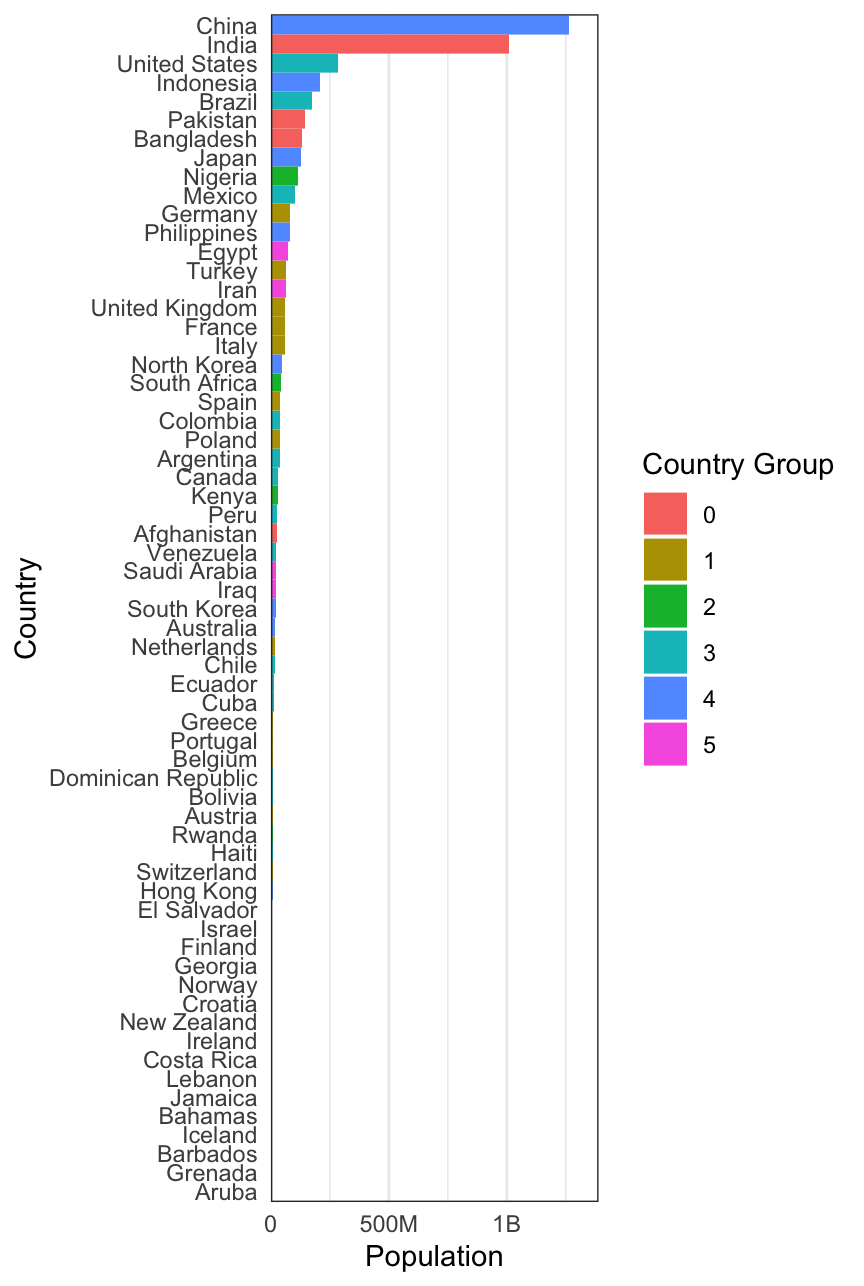
\includegraphics{hw3_files/figure-latex/unnamed-chunk-16-1.pdf}

\begin{enumerate}
\def\labelenumi{\alph{enumi}.}
\setcounter{enumi}{1}
\tightlist
\item
  Design a plot and a dynamic query so that clicking or brushing on the
  plot updates the points that are highlighted in the scatterplot in
  (a). For example, you may query a histogram of prices to focus on
  neighborhoods that are more or less affordable.
\end{enumerate}

A scatter plot of log\_price and reviews\_per\_month. Users can brush on
the plot to choose those apartment they are interested in, and the
scatter plot will highlight those chosen apartment.

\begin{enumerate}
\def\labelenumi{\alph{enumi}.}
\setcounter{enumi}{2}
\tightlist
\item
  Implement the reverse graphical query. That is, allow the user to
  update the plot in (b) by brushing over the scatterplot in (a).
\end{enumerate}

\begin{Shaded}
\begin{Highlighting}[]
\CommentTok{\# reset\_selected \textless{}{-} function(df, brush) \{}
\CommentTok{\#   brushedPoints(df,brush,allRows = TRUE)$selected\_}
\CommentTok{\# \}}
\CommentTok{\# }
\CommentTok{\# scatter\_plot \textless{}{-} function(df,selected, xvar, yvar) \{}
\CommentTok{\#   df \%\textgreater{}\% }
\CommentTok{\#     mutate(selected\_ = selected) \%\textgreater{}\%}
\CommentTok{\#     ggplot(aes\_string(x = xvar, y = yvar)) +}
\CommentTok{\#     geom\_point(aes(alpha = as.numeric(selected\_), col = room\_type)) +}
\CommentTok{\#     scale\_alpha\_continuous(range = c(0.01,1))}
\CommentTok{\# \}}
\CommentTok{\# }
\CommentTok{\# }
\CommentTok{\# ui \textless{}{-} fluidPage(}
\CommentTok{\#   titlePanel("Reverse Graphical Query"),}
\CommentTok{\#   }
\CommentTok{\#   fluidRow(}
\CommentTok{\#     column(6, plotOutput("scatter1", brush = "plot\_brush")),}
\CommentTok{\#     column(6, plotOutput("scatter2", brush = "plot\_brush"))}
\CommentTok{\#   )}
\CommentTok{\# )}
\CommentTok{\# }
\CommentTok{\# server \textless{}{-} function(input, output) \{}
\CommentTok{\#   selected \textless{}{-} reactiveVal(rep(TRUE,nrow(NYCrentals)))}
\CommentTok{\#   }
\CommentTok{\#   observeEvent(}
\CommentTok{\#     input$plot\_brush,}
\CommentTok{\#     selected(reset\_selected(NYCrentals,input$plot\_brush))}
\CommentTok{\#   )}
\CommentTok{\#   }
\CommentTok{\#   output$scatter1 \textless{}{-} renderPlot(}
\CommentTok{\#     scatter\_plot(NYCrentals,selected(), xvar = "longitude", yvar = "latitude")}
\CommentTok{\#   )}
\CommentTok{\#   output$scatter2 \textless{}{-} renderPlot(}
\CommentTok{\#     scatter\_plot(NYCrentals,selected(), xvar = "log\_price", yvar = "number\_of\_reviews")}
\CommentTok{\#   )}
\CommentTok{\# \}}
\CommentTok{\# }
\CommentTok{\# shinyApp(ui, server)}
\end{Highlighting}
\end{Shaded}

\begin{figure}
\centering
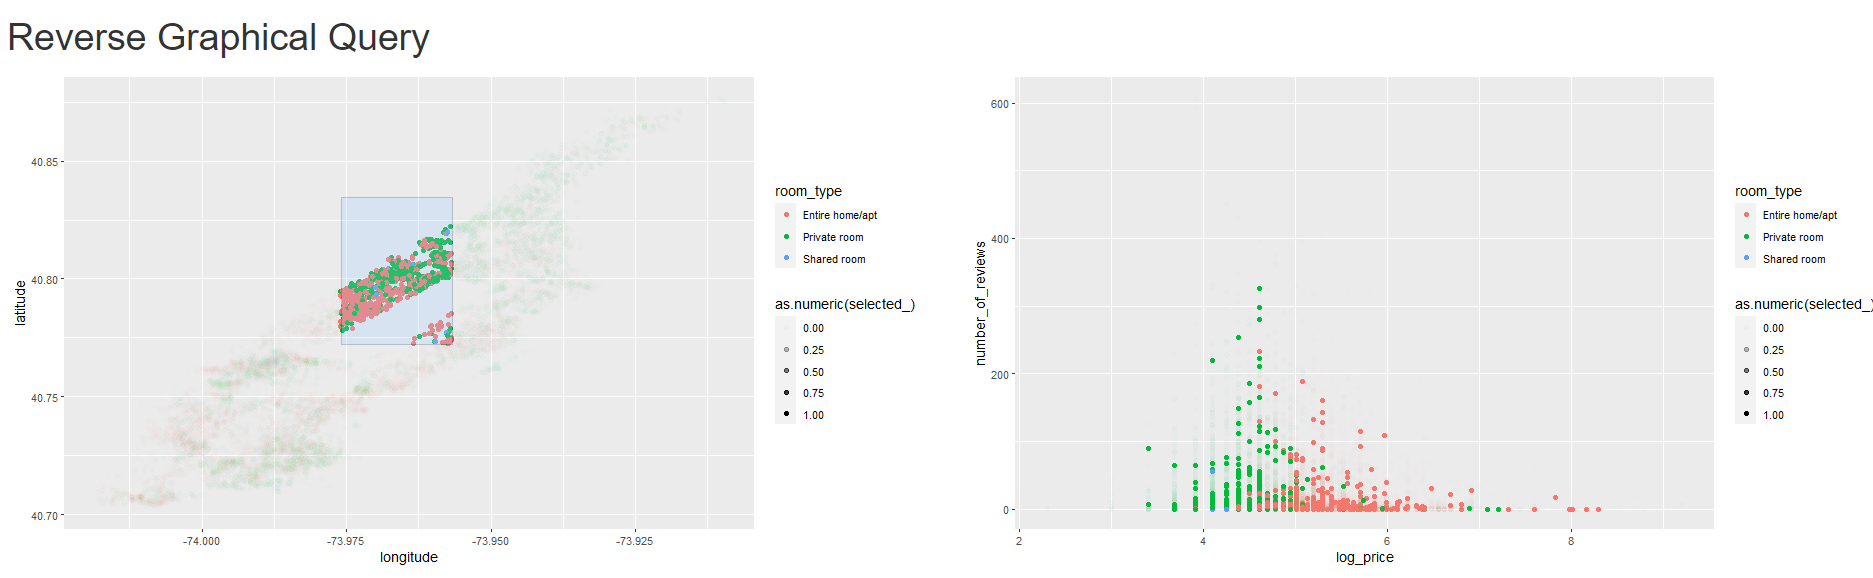
\includegraphics{Shiny1.png}
\caption{Shiny1}
\end{figure}

\begin{enumerate}
\def\labelenumi{\alph{enumi}.}
\setcounter{enumi}{3}
\tightlist
\item
  Comment on the resulting visualization(s). If you had a friend who was
  interested in renting an Airbnb in NYC, what would you tell them?
\end{enumerate}

They can choose rentals within certain range of price and how popular
the rantals are, then they can know the location of chosen rooms. To sum
up, the shiny app above provide a way that users can choose certain
range of price, and visit or rent the most popular rantal.

\#\#\#5. {[}Geospatial Datasets{]} For each of the datasets below,
specify whether it is in a vector or raster data format. If it is in a
vector data format, explain which types of geometries it contains (e.g.,
a point or linestring). Explain your reasoning.

\begin{enumerate}
\def\labelenumi{\alph{enumi}.}
\tightlist
\item
  \href{https://uwmadison.box.com/shared/static/qfmrp9srsoq0a7oj0e7xmgu5spojr33e.geojson}{NYC
  Building Footprints}
\end{enumerate}

This dataset is a vector dataset which contains polygons information. we
can use st\_geometry\_type function to check which type of geometries
this dataset contains. Another reason is that the dataset is stored in
.geojson file.

\begin{Shaded}
\begin{Highlighting}[]
\NormalTok{NYC }\OtherTok{\textless{}{-}} \FunctionTok{read\_sf}\NormalTok{(}\StringTok{"https://uwmadison.box.com/shared/static/qfmrp9srsoq0a7oj0e7xmgu5spojr33e.geojson"}\NormalTok{)}
\NormalTok{NYC}
\end{Highlighting}
\end{Shaded}

\begin{verbatim}
## Simple feature collection with 2726 features and 0 fields
## Geometry type: MULTIPOLYGON
## Dimension:     XY
## Bounding box:  xmin: -74.0048 ymin: 40.7032 xmax: -73.9648 ymax: 40.7432
## Geodetic CRS:  WGS 84
## # A tibble: 2,726 x 1
##                                                                         geometry
##                                                               <MULTIPOLYGON [°]>
##  1 (((-73.99587 40.7432, -73.99348 40.74228, -73.99381 40.74179, -73.99639 40.7~
##  2 (((-74.00315 40.73253, -74.00318 40.73254, -74.00319 40.73255, -74.0031 40.7~
##  3 (((-74.00129 40.72418, -74.00212 40.72305, -74.00277 40.72332, -74.00209 40.~
##  4 (((-73.99679 40.7239, -73.99631 40.7246, -73.99603 40.72449, -73.99652 40.72~
##  5 (((-73.99473 40.72505, -73.99445 40.72575, -73.99433 40.72573, -73.99437 40.~
##  6 (((-73.99951 40.73009, -74.00019 40.72914, -74.00052 40.72927, -74.00047 40.~
##  7 (((-73.992 40.7274, -73.99214 40.72745, -73.99202 40.72761, -73.99192 40.727~
##  8 (((-73.98689 40.714, -73.98707 40.71399, -73.98709 40.71422, -73.98691 40.71~
##  9 (((-73.99174 40.71495, -73.9913 40.71594, -73.99069 40.71578, -73.99113 40.7~
## 10 (((-73.99187 40.71858, -73.99223 40.71778, -73.99293 40.71796, -73.99257 40.~
## # i 2,716 more rows
\end{verbatim}

\begin{enumerate}
\def\labelenumi{\alph{enumi}.}
\setcounter{enumi}{1}
\tightlist
\item
  \href{https://github.com/krisrs1128/stat479_s22/blob/main/_slides/week7/exercises/data/afripop2020.tif?raw=true}{Africa
  Population 2020}
\end{enumerate}

It is a raster dataset, which is stored in .tif file. We can also find
the data format by the decription below.

\begin{Shaded}
\begin{Highlighting}[]
\NormalTok{Africa }\OtherTok{\textless{}{-}} \FunctionTok{rast}\NormalTok{(}\StringTok{"https://github.com/krisrs1128/stat479\_s22/blob/main/\_slides/week7/exercises/data/afripop2020.tif?raw=true"}\NormalTok{)}
\NormalTok{Africa}
\end{Highlighting}
\end{Shaded}

\begin{verbatim}
## class       : SpatRaster 
## dimensions  : 434, 413, 1  (nrow, ncol, nlyr)
## resolution  : 0.1666667, 0.1666667  (x, y)
## extent      : -17.62625, 51.20708, -34.97542, 37.35792  (xmin, xmax, ymin, ymax)
## coord. ref. : lon/lat WGS 84 (EPSG:4326) 
## source      : afripop2020.tif?raw=true 
## varname     : afripop2020 
## name        : afripop2020 
## min value   :        0.00 
## max value   :    21181.16
\end{verbatim}

\begin{enumerate}
\def\labelenumi{\alph{enumi}.}
\setcounter{enumi}{2}
\tightlist
\item
  \href{https://github.com/krisrs1128/stat479_s22/tree/main/_slides/week7/exercises/data/glacial_lakes}{Himalayan
  Glacial Lakes} It is a vector data set in polygon format, because in
  geometry column it contains ``polygon''
\end{enumerate}

\begin{Shaded}
\begin{Highlighting}[]
\NormalTok{Himalayan }\OtherTok{\textless{}{-}} \FunctionTok{read\_sf}\NormalTok{(}\StringTok{"C:}\SpecialCharTok{\textbackslash{}\textbackslash{}}\StringTok{Users}\SpecialCharTok{\textbackslash{}\textbackslash{}}\StringTok{12927}\SpecialCharTok{\textbackslash{}\textbackslash{}}\StringTok{Desktop}\SpecialCharTok{\textbackslash{}\textbackslash{}}\StringTok{visiting}\SpecialCharTok{\textbackslash{}\textbackslash{}}\StringTok{Courses}\SpecialCharTok{\textbackslash{}\textbackslash{}}\StringTok{STAT 436}\SpecialCharTok{\textbackslash{}\textbackslash{}}\StringTok{hw3}\SpecialCharTok{\textbackslash{}\textbackslash{}}\StringTok{glacial\_lakes}\SpecialCharTok{\textbackslash{}\textbackslash{}}\StringTok{glacial\_lakes}\SpecialCharTok{\textbackslash{}\textbackslash{}}\StringTok{GL\_3basins\_2015.shp"}\NormalTok{)}
\NormalTok{Himalayan}
\end{Highlighting}
\end{Shaded}

\begin{verbatim}
## Simple feature collection with 3624 features and 10 fields
## Geometry type: POLYGON
## Dimension:     XY
## Bounding box:  xmin: 80.07264 ymin: 27.43573 xmax: 88.71977 ymax: 30.62196
## Geodetic CRS:  WGS 84
## # A tibble: 3,624 x 11
##       Id Latitude Longitude GL_ID Basin Sub_Basin   Area Elevation Type  Country
##    <dbl>    <dbl>     <dbl> <chr> <chr> <chr>      <dbl>     <dbl> <chr> <chr>  
##  1     1     28.9      86.5 GL08~ Koshi Arun      0.917       5098 E(o)  China  
##  2     2     28.9      86.5 GL08~ Koshi Arun      0.866       5254 E(o)  China  
##  3     3     28.8      87.5 GL08~ Koshi Arun      0.0427      5402 E(o)  China  
##  4     4     28.8      86.5 GL08~ Koshi Arun      2.82        5319 E(o)  China  
##  5     5     28.8      87.5 GL08~ Koshi Arun      0.0789      5453 E(o)  China  
##  6     6     28.8      87.5 GL08~ Koshi Arun      0.0426      5495 E(o)  China  
##  7     7     28.8      87.6 GL08~ Koshi Arun      0.0593      5642 E(o)  China  
##  8     8     28.8      87.4 GL08~ Koshi Arun      0.211       5551 E(o)  China  
##  9     9     28.8      87.6 GL08~ Koshi Arun      0.273       5316 E(o)  China  
## 10    10     28.8      87.6 GL08~ Koshi Arun      0.0557      5760 E(o)  China  
## # i 3,614 more rows
## # i 1 more variable: geometry <POLYGON [°]>
\end{verbatim}

\begin{enumerate}
\def\labelenumi{\alph{enumi}.}
\setcounter{enumi}{3}
\tightlist
\item
  \href{https://raw.githubusercontent.com/krisrs1128/stat479_s22/main/_slides/week7/exercises/data/ev.geojson}{US
  EV Charging}
\end{enumerate}

This is a dataset in point format according to the decription below.
Also, another reason is that the dataset is stored in .geojson file.

\begin{Shaded}
\begin{Highlighting}[]
\NormalTok{US }\OtherTok{\textless{}{-}} \FunctionTok{read\_sf}\NormalTok{(}\StringTok{"https://raw.githubusercontent.com/krisrs1128/stat479\_s22/main/\_slides/week7/exercises/data/ev.geojson"}\NormalTok{)}
\NormalTok{US}
\end{Highlighting}
\end{Shaded}

\begin{verbatim}
## Simple feature collection with 846 features and 68 fields
## Geometry type: POINT
## Dimension:     XY
## Bounding box:  xmin: -92.75408 ymin: 42.51329 xmax: -87.02122 ymax: 46.94643
## Geodetic CRS:  WGS 84
## # A tibble: 846 x 69
##    OBJECTID FUEL_TYPE_ STATION_NA  STREET_ADD INTERSECTI CITY  STATE ZIP   PLUS4
##       <int> <chr>      <chr>       <chr>      <chr>      <chr> <chr> <chr> <chr>
##  1      235 LPG        AmeriGas    700 Count~ Route 12 ~ Elkh~ WI    53121 <NA> 
##  2      287 LPG        AmeriGas    4117 Term~ Near High~ McFa~ WI    53558 <NA> 
##  3      288 LPG        Ferrellgas  1301 S St~ <NA>       Madi~ WI    53716 <NA> 
##  4      289 LPG        Roche-A-Cr~ 503 S Mai~ Highway 1~ Adams WI    53910 <NA> 
##  5      290 LPG        United Co-~ 7160 N Ra~ 0.5 mile ~ Beav~ WI    53916 <NA> 
##  6      291 LPG        Lakes Gas ~ 50 Packer~ Off Highw~ Robe~ WI    54023 <NA> 
##  7      292 LPG        Ferrellgas  801 Prosp~ East on C~ Osce~ WI    54020 <NA> 
##  8      293 LPG        Superior G~ 212 W 14t~ 1.5 block~ Mars~ WI    54449 <NA> 
##  9      294 LPG        AmeriGas    112 S Par~ Near High~ Rhin~ WI    54501 <NA> 
## 10      295 LPG        Midland Se~ 411 Sanbo~ From the ~ Ashl~ WI    54806 <NA> 
## # i 836 more rows
## # i 60 more variables: STATION_PH <chr>, STATUS_COD <chr>, EXPECTED_D <date>,
## #   GROUPS_WIT <chr>, ACCESS_DAY <chr>, CARDS_ACCE <chr>, BD_BLENDS <chr>,
## #   NG_FILL_TY <chr>, NG_PSI <chr>, EV_LEVEL1_ <chr>, EV_LEVEL2_ <chr>,
## #   EV_DC_FAST <chr>, EV_OTHER_I <chr>, EV_NETWORK <chr>, EV_NETWO_1 <chr>,
## #   GEOCODE_ST <chr>, LATITUDE <dbl>, LONGITUDE <dbl>, DATE_LAST_ <date>,
## #   ID <int>, UPDATED_AT <date>, OWNER_TYPE <chr>, FEDERAL_AG <chr>, ...
\end{verbatim}

\begin{enumerate}
\def\labelenumi{\alph{enumi}.}
\setcounter{enumi}{4}
\tightlist
\item
  \href{https://github.com/krisrs1128/stat479_s22/blob/main/_slides/week7/exercises/data/landsat.tif?raw=true}{Zion
  Elevation} This is a raster dataset which is stored in .tif file.
  Another reason is as following code.
\end{enumerate}

\begin{Shaded}
\begin{Highlighting}[]
\NormalTok{Zion }\OtherTok{\textless{}{-}} \FunctionTok{rast}\NormalTok{(}\StringTok{"https://github.com/krisrs1128/stat479\_s22/blob/main/\_slides/week7/exercises/data/landsat.tif?raw=true"}\NormalTok{)}
\NormalTok{Zion}
\end{Highlighting}
\end{Shaded}

\begin{verbatim}
## class       : SpatRaster 
## dimensions  : 1428, 1128, 4  (nrow, ncol, nlyr)
## resolution  : 30, 30  (x, y)
## extent      : 301905, 335745, 4111245, 4154085  (xmin, xmax, ymin, ymax)
## coord. ref. : WGS 84 / UTM zone 12N (EPSG:32612) 
## source      : landsat.tif?raw=true 
## varname     : landsat 
## names       : landsat_1, landsat_2, landsat_3, landsat_4 
## min values  :      7550,      6404,      5678,      5252 
## max values  :     19071,     22051,     25780,     31961
\end{verbatim}

\#\#\#6. {[}Olympics Interactive App{]} The code below sets up a Shiny
app for interactively visualizing athlete weight and heights in the 2012
London Olympics. We would like to have an interactive scatterplot of
\texttt{Weight} vs. \texttt{Height,\ cm} that updates which points
(athletes) are highlighted depending on which sports have been selected
by a dropdown menu. Code for generating the scatterplot is provided in
the function \texttt{scatterplot}.

\begin{Shaded}
\begin{Highlighting}[]
\CommentTok{\# library(shiny)}
\CommentTok{\# library(tidyverse)}
\CommentTok{\# olympics \textless{}{-} read.csv("https://uwmadison.box.com/shared/static/rzw8h2x6dp5693gdbpgxaf2koqijo12l.csv")}
\CommentTok{\# }
\CommentTok{\# \#\textquotesingle{} Scatterplot with highlighted points}
\CommentTok{\# \#\textquotesingle{}}
\CommentTok{\# \#\textquotesingle{} Assumes a column in df called "selected" saying whether points should be}
\CommentTok{\# \#\textquotesingle{} larger / darker}
\CommentTok{\# scatterplot \textless{}{-} function(df) \{}
\CommentTok{\#   ggplot(df) +}
\CommentTok{\#     geom\_point(aes(}
\CommentTok{\#       Weight,}
\CommentTok{\#       Height..cm,}
\CommentTok{\#       alpha = as.numeric(selected),}
\CommentTok{\#       size = as.numeric(selected)}
\CommentTok{\#     )) +}
\CommentTok{\#     scale\_alpha(range = c(0.05, .8)) +}
\CommentTok{\#     scale\_size(range = c(0.1, 1))}
\CommentTok{\# \}}
\CommentTok{\# }
\CommentTok{\# ui \textless{}{-} fluidPage(}
\CommentTok{\#   selectInput(}
\CommentTok{\#     "dropdown",}
\CommentTok{\#     "Select a Sport",}
\CommentTok{\#     choices = unique(olympics$Sport),}
\CommentTok{\#     multiple = TRUE}
\CommentTok{\#   ),}
\CommentTok{\#   plotOutput("scatterplot")}
\CommentTok{\# )}
\CommentTok{\# }
\CommentTok{\# server \textless{}{-} function(input, output) \{}
\CommentTok{\#   \# fill this in...}
\CommentTok{\#   }
\CommentTok{\#   output$scatterplot \textless{}{-} renderPlot(\{olympics \%\textgreater{}\%}
\CommentTok{\#                                      mutate(selected = Sport \%in\% input$dropdown) \%\textgreater{}\%}
\CommentTok{\#                                      scatterplot()\})}
\CommentTok{\# \}}
\end{Highlighting}
\end{Shaded}

\begin{enumerate}
\def\labelenumi{\alph{enumi}.}
\tightlist
\item
  Provide server code which would allow the scatterplot to update the
  highlighted athletes depending on the currently selected sports.
\end{enumerate}

\begin{figure}
\centering
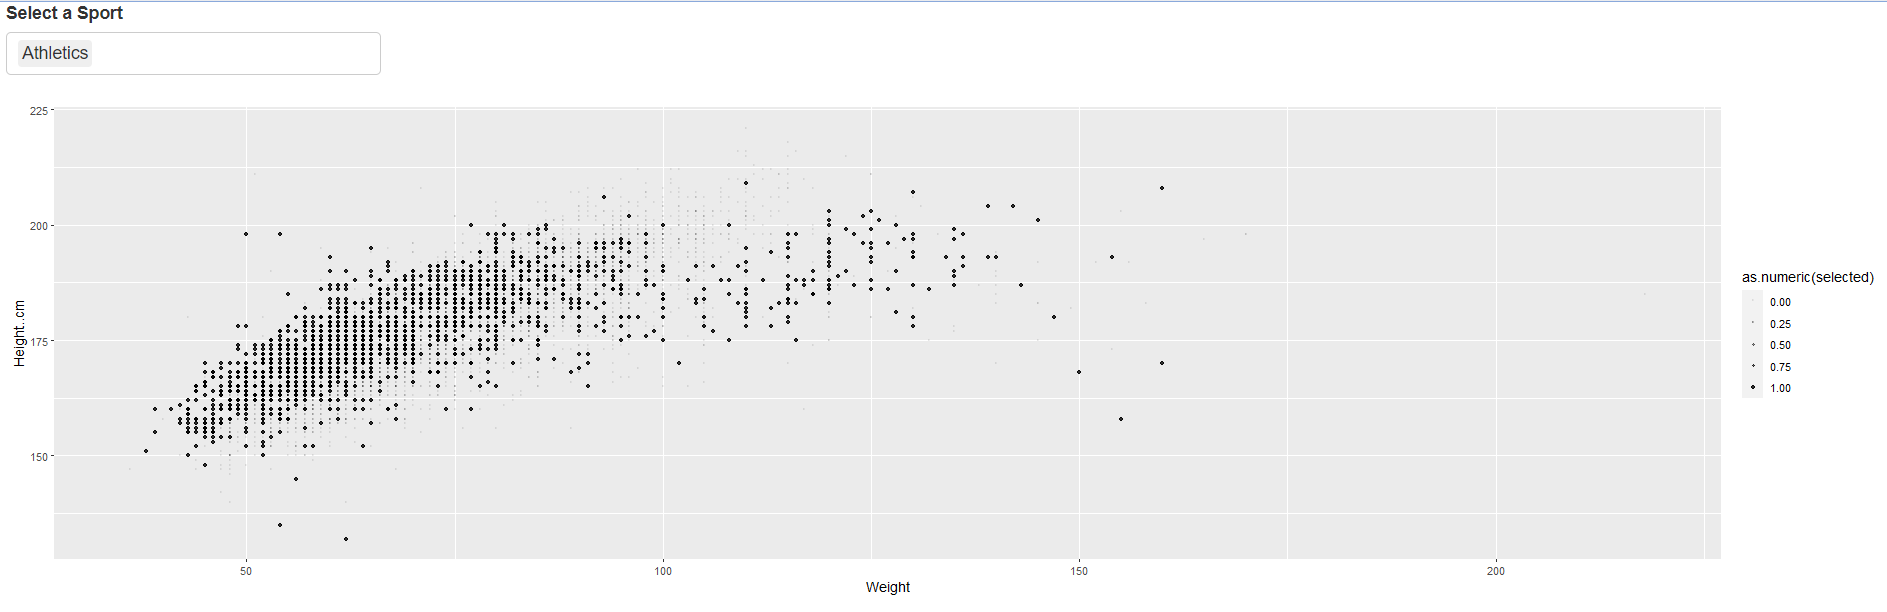
\includegraphics{Shiny2.png}
\caption{Shiny2}
\end{figure}

\begin{Shaded}
\begin{Highlighting}[]
\CommentTok{\# shinyApp(ui,server)}
\end{Highlighting}
\end{Shaded}

\begin{enumerate}
\def\labelenumi{\alph{enumi}.}
\setcounter{enumi}{1}
\item
  We have been asked to also print a table of the selected athletes.
  Assume the UI has the form,

\begin{Shaded}
\begin{Highlighting}[]
\CommentTok{\# ui \textless{}{-} fluidPage(}
\CommentTok{\#   selectInput("dropdown", "Select a Sport", choices = unique(olympics$Sport), multiple = TRUE),}
\CommentTok{\#   plotOutput("scatterplot"),}
\CommentTok{\#   dataTableOutput("table") }
\CommentTok{\# )}
\end{Highlighting}
\end{Shaded}
\end{enumerate}

Describe changes to your solution to (a) to meet the new requirements.
How would you minimize code duplication? Be as specific as possible.

\begin{enumerate}
\def\labelenumi{\arabic{enumi}.}
\tightlist
\item
  Add an reactive expression to dynamically select the required
  athletes.
\item
  use ``renderTable'' function to ouput the result of the table. Brief
  Code:
\end{enumerate}

\begin{Shaded}
\begin{Highlighting}[]
\CommentTok{\# server \textless{}{-} function(input, output) \{}
\CommentTok{\#   }\AlertTok{\#\#\#}\CommentTok{ other code }\AlertTok{\#\#\#}
\CommentTok{\#   selected\_athlete \textless{}{-} reactive (\{}
\CommentTok{\#     olympics \%\textgreater{}\%}
\CommentTok{\#       mutate(selected = Sport \%in\% input$dropdown)}
\CommentTok{\#   \})}
\CommentTok{\#   }\AlertTok{\#\#\#}\CommentTok{ other code }\AlertTok{\#\#\#}
\CommentTok{\#   }
\CommentTok{\#   output$table \textless{}{-} renderTable(selected\_athlete)}
\CommentTok{\#   }\AlertTok{\#\#\#}\CommentTok{ other code }\AlertTok{\#\#\#}
\CommentTok{\# \}}
\end{Highlighting}
\end{Shaded}


\end{document}
